\documentclass[a4paper, 11pt, oneside]{article}

\usepackage[utf8]{inputenc}
\usepackage[T1]{fontenc}
\usepackage[english]{babel}
\usepackage{array}
\usepackage{shortvrb}
\usepackage{listings}
\usepackage[fleqn]{amsmath}
\usepackage{amsfonts}
\usepackage{fullpage}
\usepackage{enumerate}
\usepackage{graphicx}
\usepackage{alltt}
\usepackage{indentfirst}
\usepackage{eurosym}
\usepackage{titlesec, blindtext, color}
\usepackage[table,xcdraw,dvipsnames]{xcolor}
\usepackage[unicode]{hyperref}
\usepackage{url}
\usepackage{float}
\usepackage{subcaption}
\usepackage[skip=1ex]{caption}
\definecolor{brightpink}{rgb}{1.0, 0.0, 0.5}

\usepackage{titling}
\renewcommand\maketitlehooka{\null\mbox{}\vfill}
\renewcommand\maketitlehookd{\vfill\null}

\newcommand{\ClassName}{ELEN-0060: Information and Coding Theory}
\newcommand{\ProjectName}{Project 2 - Source coding, data compression, and \\ channel coding}
\newcommand{\AcademicYear}{2021 - 2022}

%%%% First page settings %%%%

\title{\ClassName\\\vspace*{0.8cm}\ProjectName\vspace{1cm}}
\author{Maxime Goffart \\180521 \and Olivier Joris\\182113}
\date{\vspace{1cm}Academic year \AcademicYear}

\begin{document}

%%% First page %%%
\begin{titlingpage}
{\let\newpage\relax\maketitle}
\end{titlingpage}

\thispagestyle{empty}
\newpage

%%%%%%%%%%%%%%%%%%%%%%%%%%%%%%%%%%%%%%%%%%

%%% Table of contents %%%
%\tableofcontents
%\newpage

%%%%%%%%%%%%%%%%%%%%%%%%%%%%%%%%%%%%%%%%%%

% CONTENT %
\section{Implementation}

% Implement a function that returns a binary Huffman code for a given probability
% distribution. Give the main steps of your implementation. Verify your code on
% Exercise 7 of the second exercise session (TP2), and report the output of your code
% for this example. Explain how to extend your function to generate a Huffman code of
% any (output) alphabet size.
\subsection{Binary Huffman code (question 1)}
\paragraph{}Our implementation is based on a data structure representing a Node of the tree which has 4 fields: 
\begin{itemize}
\item the symbol of the Node which is 'None' if the Node is not a leaf.
\item the probability of the Node.
\item a pointer to the left child of the Node which is 'None' if the Node is a leaf.
\item a pointer to the right child of the Node which is 'None' if the Node is a leaf.
\end{itemize}

We first create a node for each letter in which we store its symbol, its probability, and 'None' for both children.
Then, we build the tree as seen in class: we iteratively link the two nodes with the lowest probabilities until the tree is complete with a node having 1 as probability at root. Each new node born from the birth of two nodes has for probability the sum of the probabilities of these nodes. It also maintains a link to these two nodes becoming its children, and has for symbol 'None'.
Finally, we recursively build the Huffman code on the basis of the previously built tree and a choice to represent a left child by a 0 and a right child by a 1.

\paragraph{}The output of our code for this question is: \texttt{\{'A': '000', 'B': '001', 'E': '01', 'C': '100', 'D': '101', 'F': '11'\}} which is not
the same as the one found during the exercise session. It is not a problem because the Huffman code is not unique. Our code is acceptable and its tree can be observed in the figure \ref{fig:huffman_tree}.

\begin{figure}[H]
    \center
    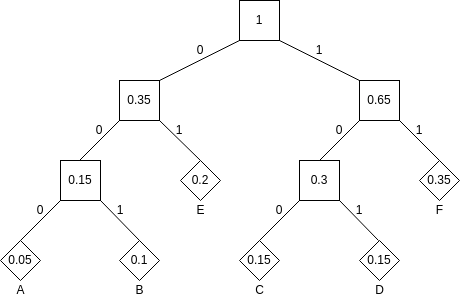
\includegraphics[scale=0.7]{huffman_tree.png}
    \caption{Huffman tree corresponding to the output code}
    \label{fig:huffman_tree}
    \end{figure}

\paragraph{}To generate a Huffman code of any (output) alphabet size, several changes would be necessary both in our data structure and in our algorithm:
\begin{itemize}
    \item Data structure
        \begin{itemize}
            \item We would need to add a field to store the alphabet size $N$ which was implicitly set to 2 in the binary Huffman code.
            \item We would need to store the $N$ children of each node which is not a leaf instead of the two children in the binary Huffman code.
        \end{itemize}
    \item Algorithm
        \begin{itemize}
            \item We would need to take the $N$ lowest probability and link them to create new nodes instead of the two nodes with the lowest probability in the binary Huffman code.
            \item We would need to assign a given unique symbol of the code to each child of a node when recursively building the Huffman code instead of 1 and 0 in the binary Huffman code where there were only 2 children per node.
            \item We might have to deal with problems of number of symbols and size of the alphabet not compatible unlike in the binary Huffman code where it is always possible to merge the two lowest probable nodes. 
        \end{itemize}
\end{itemize}

\subsection{On-line Lempel-Ziv algorithm (question 2)}

\paragraph{}The example given in the course about state of the art in data compression on slide 50/53 where the sequence 1011010100010 is encoded gives this output for our \texttt{LZ\_online} function:
\begin{itemize}
    \item Dictionary: \{'': (0, ''), '1': (1, '1'), '0': (2, '00'), '11': (3, '011'), '01': (4, '101'), '010': (5, '1000'), '00': (6, '0100'), '10': (7, '0010')\}
    \item Encoded sequence: 100011101100001000010
\end{itemize}

\subsection{Comparison between the two versions of the Lempel-Ziv algorithm (question 3)}
\paragraph{}The basic version has one main problem which is address coding. It needs to know the
size of the dictionary before an address encoding. The on-line version solves this problem by using the current dictionary size to determine the number of bits which is equal to $\lceil\log_2{N}\rceil$, where $N$ is the dictionary size. It is thus decreasing the size of the encoded text. This on-line variant is most of the time not very competitive in
terms of optimality but is very robust because it does not need assumptions about source behaviour and can thus allow an instantaneous coding without having to browse the dictionary multiple times. The asymptotic performances are reached only when the dictionary starts to become
representative: when it contains a significant fraction of sufficiently long typical messages.

\subsection{Implementation of the Lempel-Ziv 77 algorithm (question 4)}
\paragraph{}Running the example given in Figure 2 with our function and taking a \texttt{window\_size} of size 7 gives us this output: [(0, 0, 'a'), (0, 0, 'b'), (0, 0, 'r'), (3, 1, 'c'), (2, 1, 'd'), (7, 4, 'd')]. We have chosen to set the size of the look ahead buffer to the size of the window because it allows to have longer matches prefix and the prefix cannot be longer than the this size.



%%%%%%%%%%%%%%%%%%%%%%%%%%%%%%%%%%%%%%%%%%
\section{Channel coding}

\subsection{Question 16}
\paragraph{}In order to implement a function to read and display the given image, we used the methods \texttt{imread} and \texttt{imshow} provided by OpenCV.

%%%%%

\subsection{Question 17}
\paragraph{}To encode the image signal, we used a fixed-length binary code of 8 bits. We have chosen 8 bits because there are 256 (from 0 to 255) possible values, so we need $\lceil log_2(256) \rceil =8$.\\
The code is the binary representation of the grayscale value of each pixel.

%%%%%

\subsection{Question 18}
\paragraph{}By simulating the channel effect on the binary signal of the image, we get the following image:
\begin{figure}[H]
    \centering
    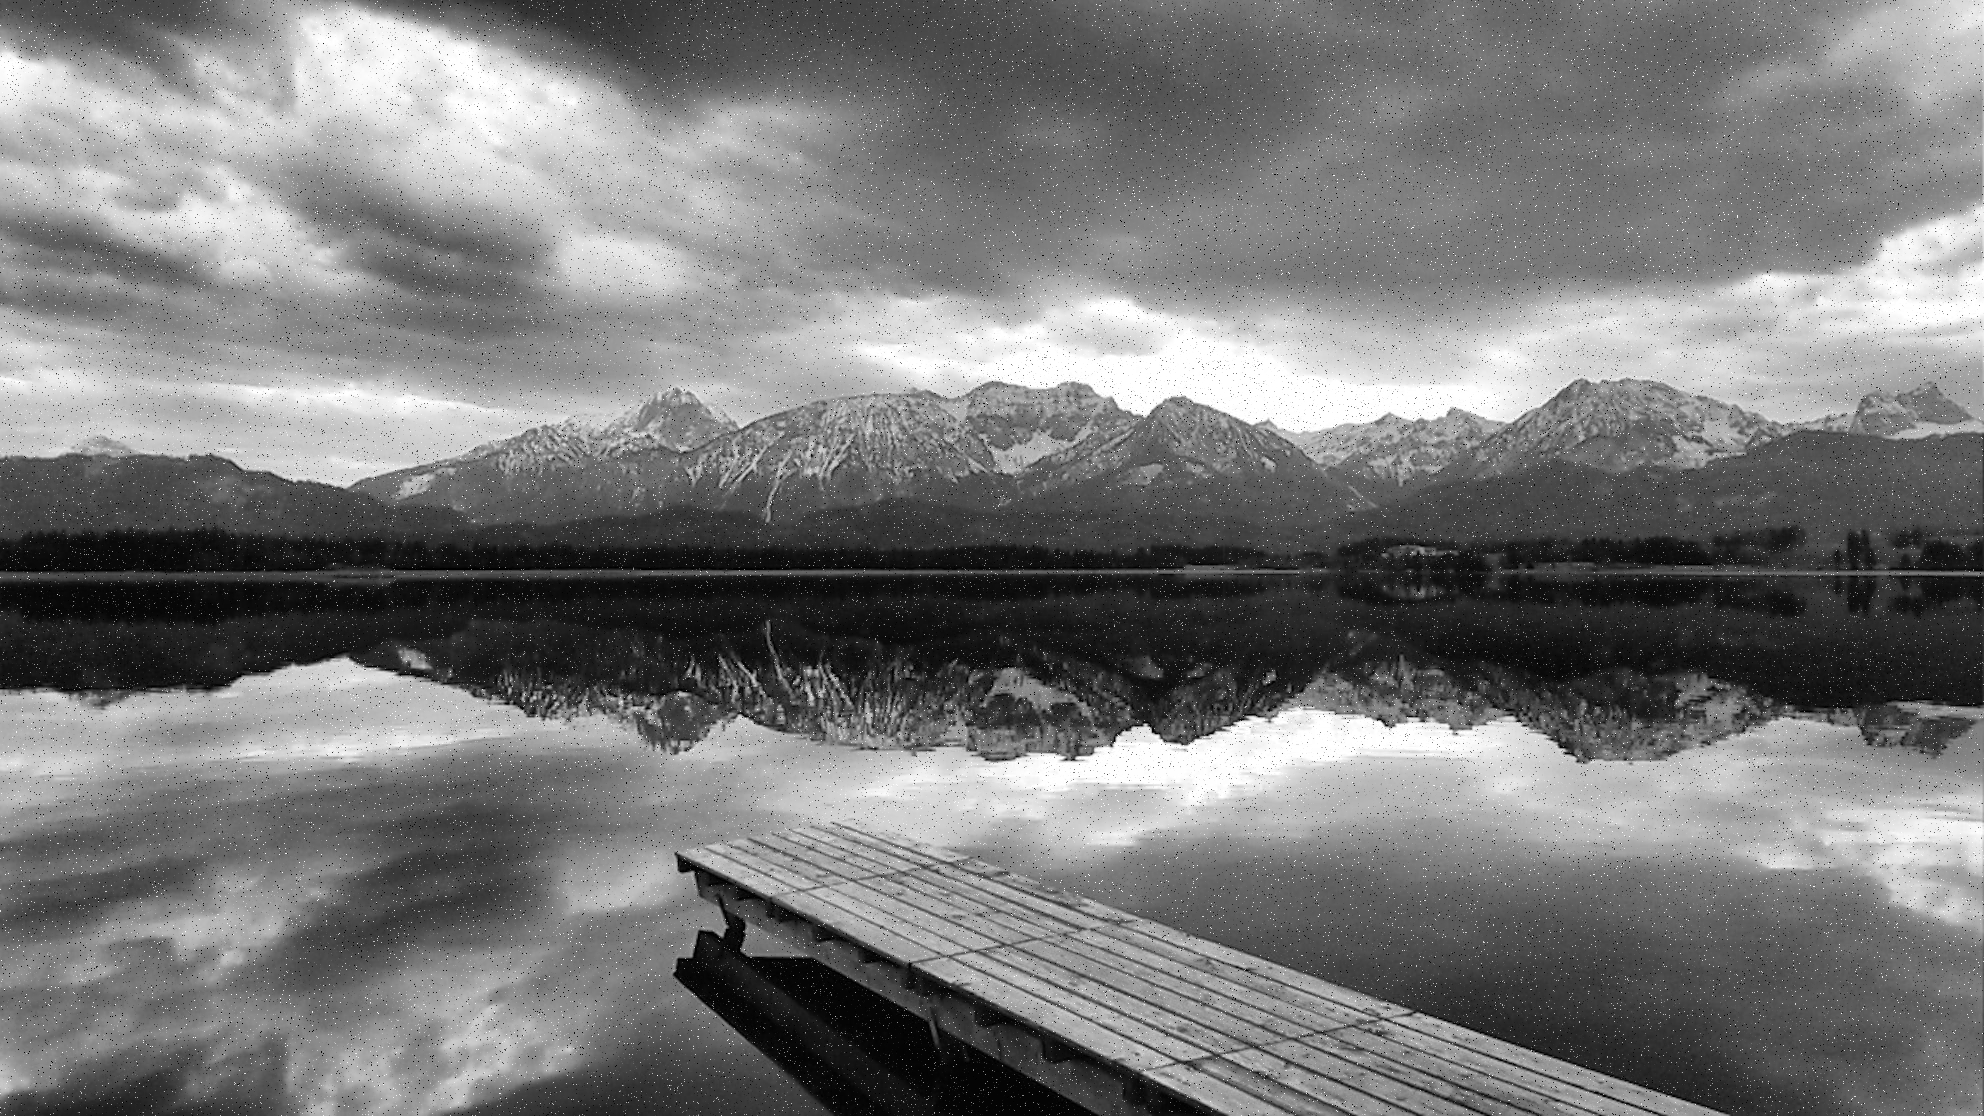
\includegraphics[scale=0.2]{q18.png}
    \caption{Image after simulating the channel effect}
\end{figure}
As we can see in the picture, after simulating the channel effect, there are a lot of small dots\footnote{Zoom in the image to see them better.} that are pixels with different grayscale values
compared to their very close neighbors.\\
This is due to the fact that we are simulating a potential loss bit by bit and we are not using any sort of redundancy.
Thus, if one of the most significant bits is modified, it completely changes the grayscale value for the pixel.

%%%%%

\subsection{Question 19}
\paragraph{}In order to compute the Hamming(7,4) code for the binary image signal, we need to add 3 redundancy bits for every 4 bits. The 3 redundancy bits are:
\begin{itemize}
    \item Bit 1 = $(bit 0 + bit 1 + bit 2) \ mod \ 2$
    \item Bit 2 = $(bit 1 + bit 2 + bit 3) \ mod \ 2$
    \item Bit 3 = $(bit 0 + bit 2 + bit 3) \ mod \ 2$
\end{itemize}
where bit 0, bit 1, bit 2, and bit 3 are, respectively, the first, second, third, and fourth bits for which we want to add redundancy.\\
By applying this principle on each block of 4 bits from the binary image signal, we get the Hamming(7,4) code for the entire binary image signal.

%%%%%

\subsection{Question 20}
\paragraph{}If we decode the binary image signal with redundancy, we get the following image:
\begin{figure}[H]
    \centering
    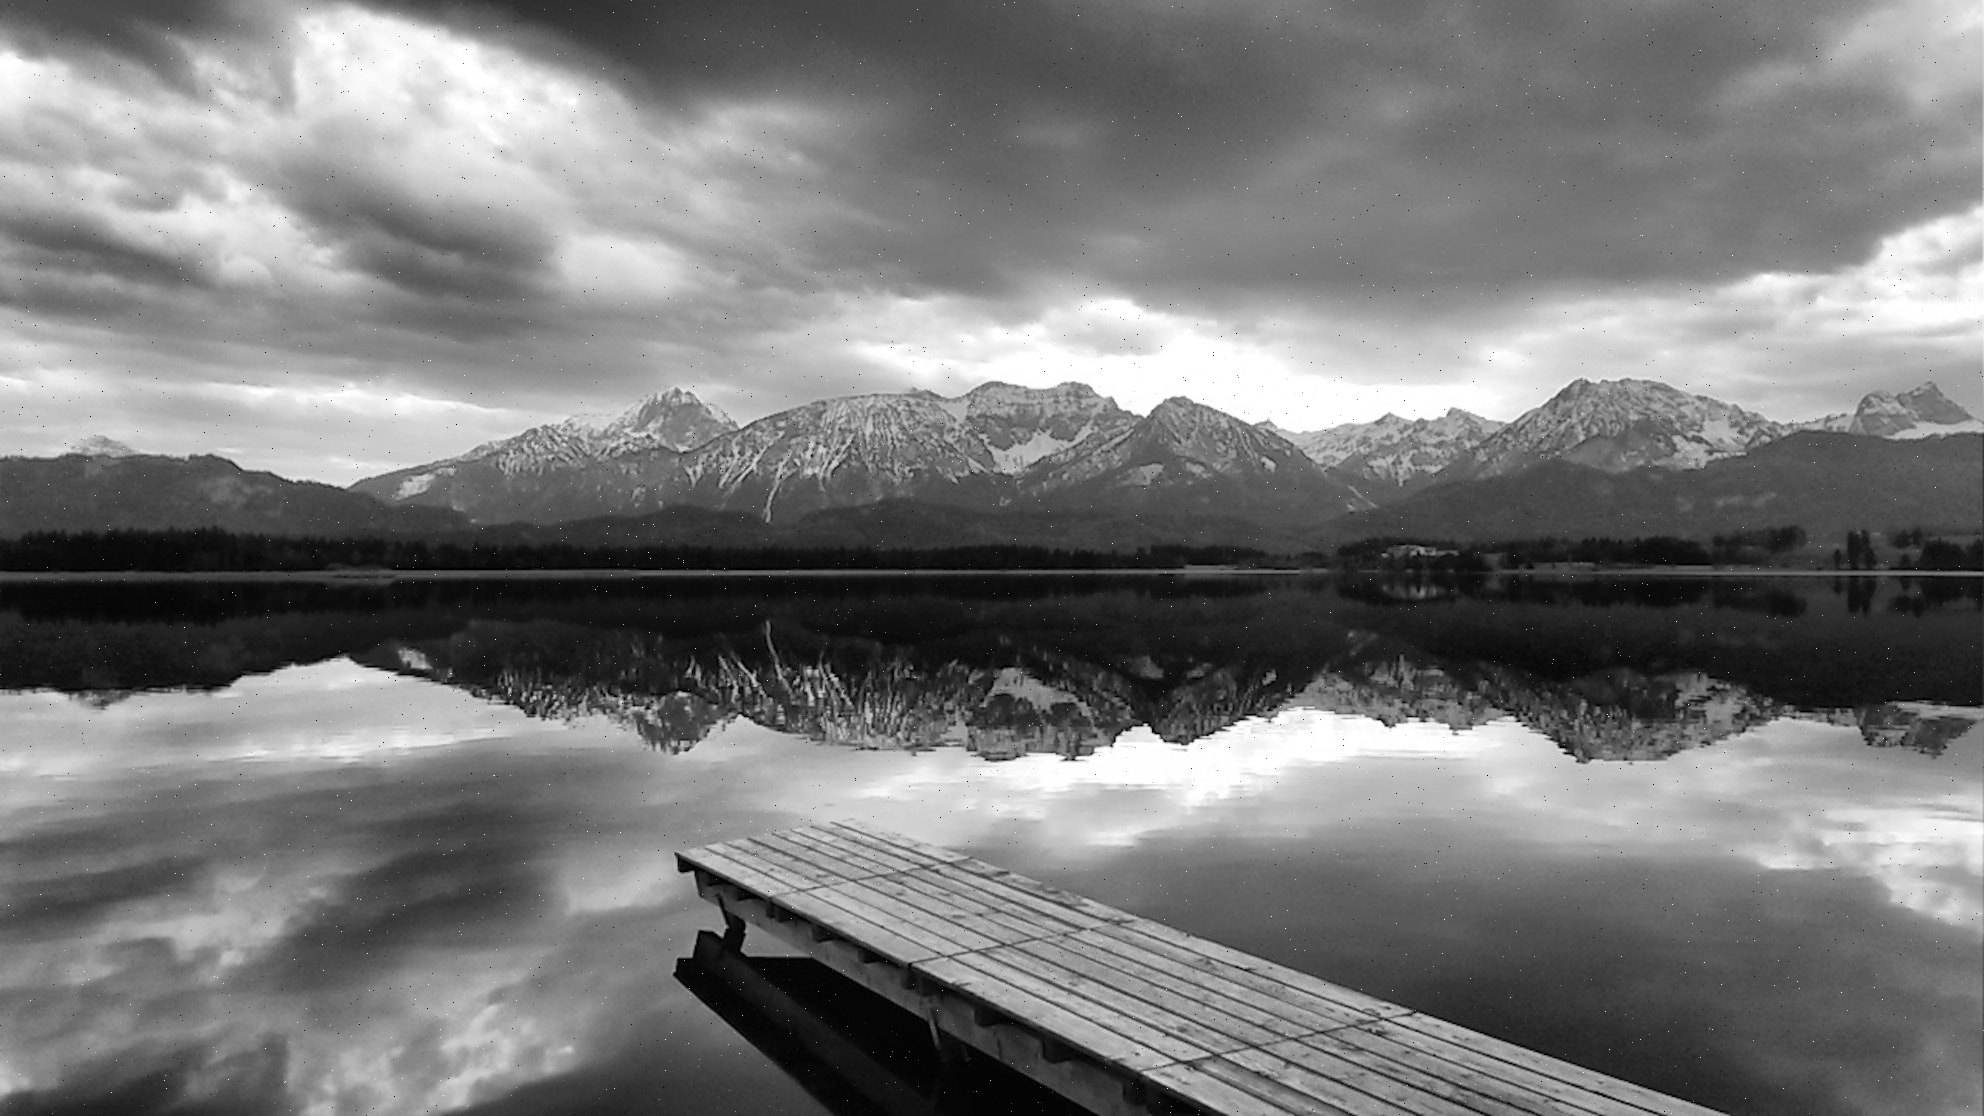
\includegraphics[scale=0.2]{q20.png}
    \caption{Image after simulating the channel effect with redundancy}
\end{figure}
As we can see in the picture, we observe less dots compared to \textit{question 18}. This is because we used redundancy with the Hamming(7,4) code.
Yet, we can still observe some dots. This is because Hamming(7,4) code can correct only one error per chunk of bits. In some cases, we might have more
than one error per chunk thus the original source is not recoverable.
\paragraph{}In order to decode the binary signal with redundancy, we used the syndrome decoding technique, as in the exercise sessions.\\
To apply this technique, we consider that the source bits were correctly transmitted through the channel. Then, we recompute the 3 parity bits based on the received 4 source bits.
Afterwards, we apply a bitwise and between the received parity bits and the re-computed parity bits.\\
Based on the result of the bitwise operation, multiple cases are possible:
\begin{itemize}
    \item If 2 or 3 bits are 1 in the result of the bitwise operation, we can deduce that one of the source bit has been incorrectly transmitted.
    To recover from the error, we can proceed the following way:
        \begin{itemize}
            \item If bits 0 and 1 of the bitwise and are 1, we need to flip the second source bit.
            \item If bits 1 and 2 of the bitwise and are 1, we need to flip the fourth source bit.
            \item If bits 0 and 2 of the bitwise and are 1, we need to flip the first source bit.
            \item If all the bits of the bitwise and are 1, we need to flip the third source bit.
        \end{itemize}
    \item If 1 bit is 1 in the result of the bitwise operation, we can deduce that one of the parity bit has been incorrectly transmitted.
    \item It is possible that 2 or more bits were transmitted incorrectly. In that case, we cannot recover from the error.
\end{itemize}

%%%%%

\subsection{Question 21}
\paragraph{}In order to reduce the loss of information, we could use Reed-Solomon codes instead of Hamming(7,4) because they allow to correct more than 1 errors
in some situations.\\
Another solution is to replace the type of channel. For instance, replacing copper wire with fiber optic in computer networks.
But, it is not also feasible.\\
There is always a trade-off between the rate and the capability of correcting from errors. Thus, in order to increase the rate,
we would need to decrease the redundancy introduced for parity.

%%%%%%%%%%%%%%%%%%%%%%%%%%%%%%%%%%%%%%%%%%

\end{document}